\documentclass[main.tex]{subfiles} % Subfile-Class

%==============================================================================%
%                                   Subfile                                    %
%==============================================================================%

\begin{document}

% Template

\subsection{Antriebe}

Der Roboter wird über 2 Schrittmotoren angetrieben. Diese bieten eine einfache
und gleichzeitig sehr präzise Möglichkeit, Lage und Position des Fahrzeugs
einzustellen. Diese Eigenschaft kommt vorallem dem Bewegungsablauf zum
umpositionieren der Hindernisse zugute, bei welchem eine genaue Position
angefahren werden muss.
Abbildung~\ref{Ansteuerungstopologie_Schrittmotorentreiber} zeigt
schematisch,wie diese Treiber angesteuert werden.

\begin{figure}[H]
    \centering
    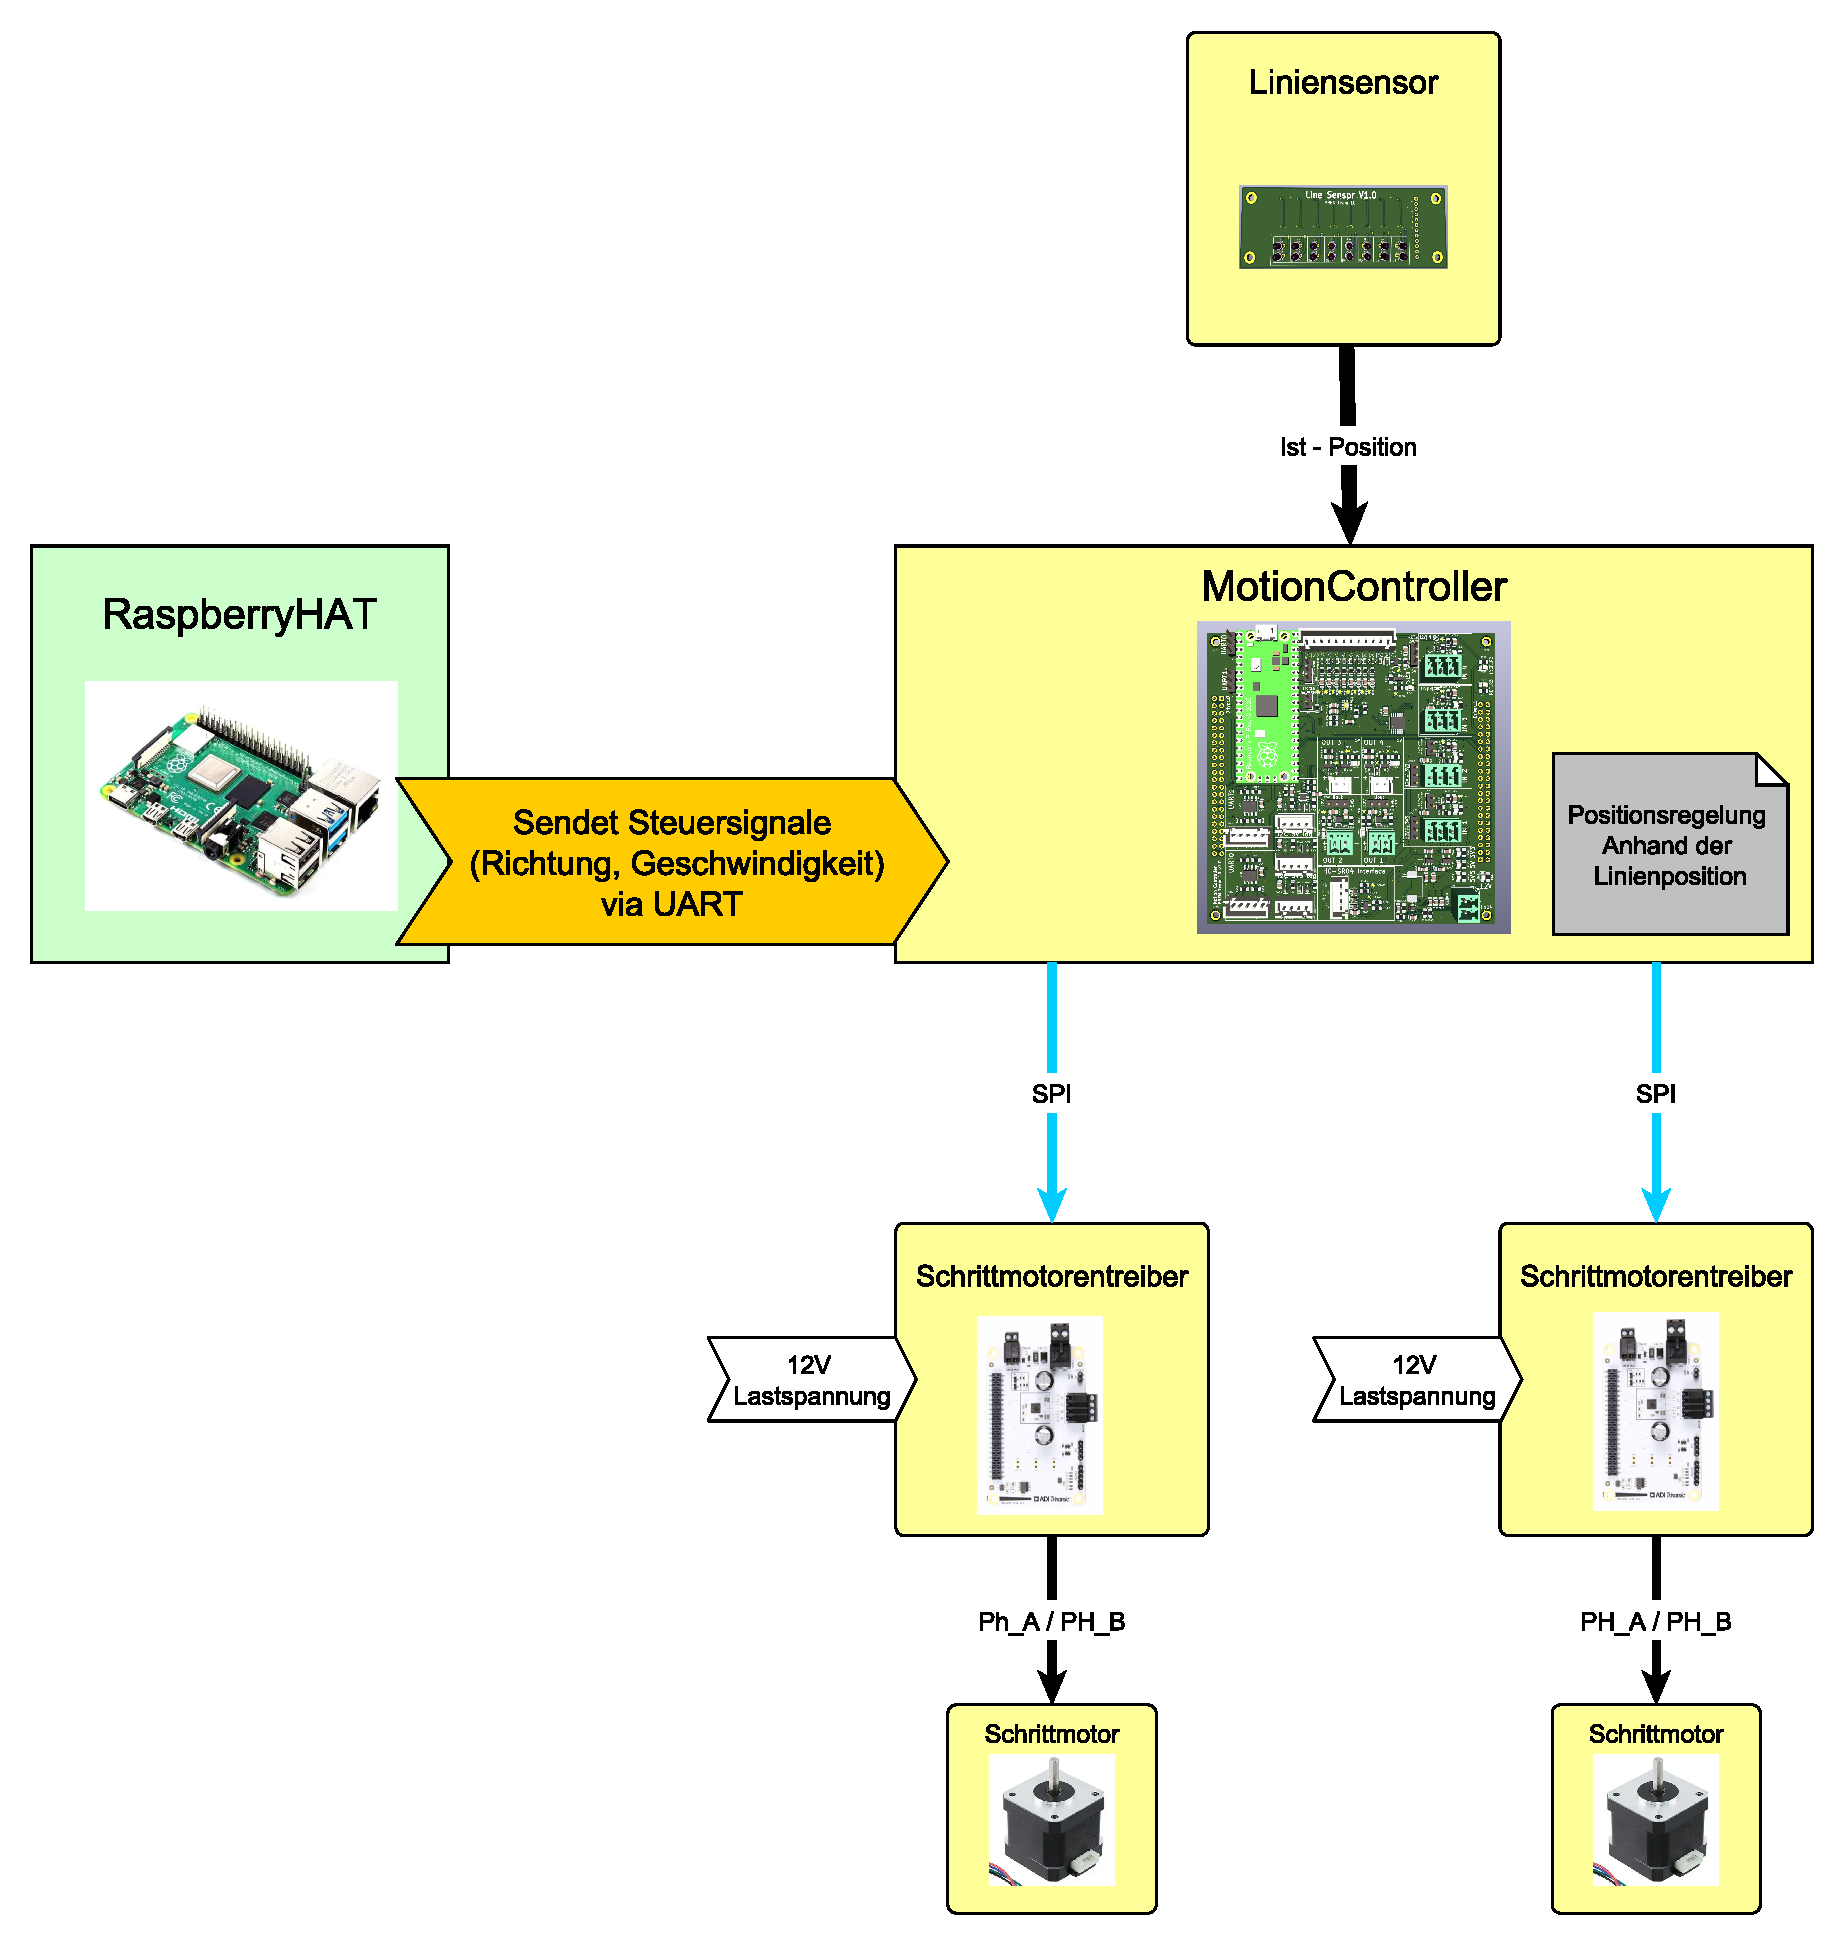
\includegraphics[width = 1\linewidth]{fig_Antriebe_und_Dimensionierung/Konzept_Motoransteuerung.pdf}
    \caption{Ansteuerungstopologie Schrittmotoren}~\label{Ansteuerungstopologie_Schrittmotorentreiber}
\end{figure}

% vgl Text aus Pren1 - kann man wahrscheinlich weitestgehend übernehmen

\subsubsection*{Motoren und Motorentreiber}

Die Ansteuerung dieser Motoren erfolgt über einen vollintegrierten
Schrittmotortreiber der Firma ADI-Trinamic. Um den Entwicklungsaufwand gering
zu halten, wird auf 2 Evaluation-Boards des Treiber-IC's \textit{TMC-5240}
zurückgegriffen, wie in Abbildung~\ref{Schrittmotorentreiber_EVAL}
gezeigt.Eines der Teammitglieder hat bereits Erfahrung mit diesem speziellen
Treiber und kann auf entsprechende Treiber-Evaluation-Boards aus seinem
beruflichen Umfeld zurückgreifen.

\subsubsection{Hardware zum Ansteuern der Antriebe}

Der MotionController wurde von vornherein darauf ausgelegt, über mehr Ein- und
Ausgänge zu verfügen als er ursprünglich gebraucht hätte. Durch diese
Designentscheidung konnte später die Aufgabe der Greifersteuerung ebenfalls
durch den MotionController übernommen werden. Für mehr Flexibilität können die
Ein- und Ausgänge auf verschiedene Spannungspegel umgeschaltet werden. Damit
können sowohl simple $3V3$ oder $5V$ Sensoren, aber auch Industrietaugliche
Sensoren und Aktoren auf 12V Spannung betrieben werden. Die Arbeitsspannung der
I2C Kommunikationsschnittstellen lässt sich ebenfalls konfigurieren sodass
zwischen $3V3$ und $5V$ Logikpegeln unterschieden werden kann. Das Gesamte
System ist damit sehr flexibel für etwaige Änderungen oder alternative
Sensoren.

Der MotionController liesst ausserdem den Liniensensor aus und regelt auf Basis
dessen die beiden Schrittmotoren. Am vorderen Ende des Fahrzeugs ist ein
Ultraschallsensor verbaut, über welchen Hindernisse auf naher Distanz (max $500
    mm$) erkannt werden. Das Umplatzieren der Hindernisse ist alleinige Aufgabe des
MotionControllers. Alle benötigte Sensorik und Aktorik ist dazu auf diesem
verbaut.

\subsubsection{Linienfolger Regelung}

Zur Regelung der Linienposition wird ein klassischer PD-Regler eingesetzt.
Fahrten, bei denen die Regelabweichung zwingend Null sein muss, sind nicht zu
erwarten, da z.B. keine Kurven exakt abgefahren werden müssen. Ein
Integralanteil ist daher nicht erforderlich.

Die Herleitung der benötigten Parameter ist im Anhang detailliert
beschrieben~\ref{apdx:Regler_Parametrierung}. Der Regler wurde zunächst mit
einem kleinen P-Anteil implementiert. In einem Experiment ist die Sprungantwort
des Systems aufgenommen und anschliessend mit regelungstechnischen Methoden zu
einem PT2-Modell modelliert. Dieses bildet die Ausgangssituation für die
Parameteridentifikation des implementierten Reglers.

Als Eingangsgrösse für den Regler dient die Linienposition, die direkt vom
Liniensensor geliefert wird. Die genaue Ermittlung dieser Grösse, wie genau der
Liniensensor ausgewertet wird, ist im Anhang
beschrieben~\ref{apdx:Liniensensor_auswertung}. Vereinfacht dargestellt werden
die einzelnen Messzellen des Sensors über einen ADC-Wandler ausgelesen, auf
einen Vektor der Grösse $0 \dots 1000$ normiert und anschliessend gewichtet
aufsummiert. Daraus ergibt sich die Position der Linie als ganzzahliger Wert
auf einer Skala von $0 \dots 7000$, wobei $3500$ die Mittenposition und damit
die Referenzposition $x[k]$ für den Regler darstellt.

\begin{figure}[H]
    \centering
    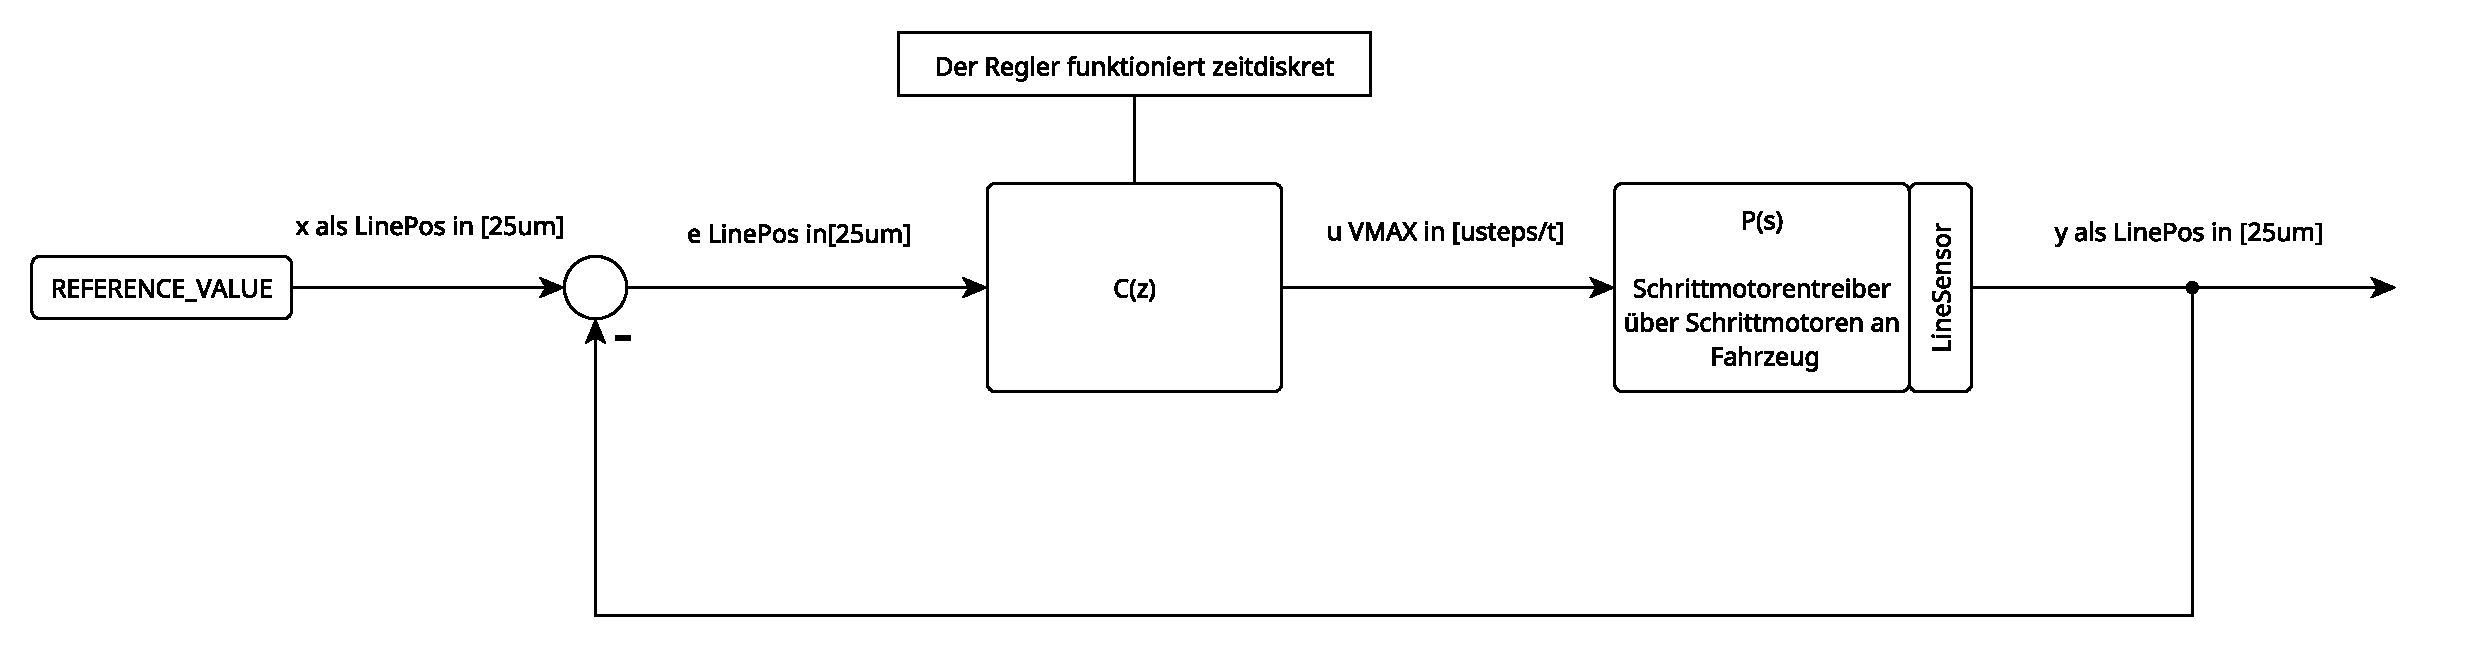
\includegraphics[width=1.0\linewidth]{../../Anhang_subfiles/Anhang_Elektronik/fig_Parametrierung_Linienfolgeregler/RegelProzess_Linienfolger.pdf}
    \caption{Reglerprozess des Linienfolgers}~\label{fig:Linienfolger_RegelProzess_ht}
\end{figure}

Der vereinfachte Regelkreis ist in
Abbildung~\ref{fig:Linienfolger_RegelProzess_ht} dargestellt. Die Grösse $x[k]$
bezeichnet, wie bereits erwähnt, die Referenzposition. Zusammen mit der
aktuellen Linienposition $y[k]$ wird die Regelabweichung $e[k]$ bestimmt. Die
Grössen in der Einheit der Linienposition ($x[k]$, $y[k]$ und $e[k]$) haben
aufgrund der Messauflösung der Zellen alle die Einheit $25 \mu m$. Der
dargestellte Block $C(z)$ repräsentiert den im MotionController implementierten
zeitdiskreten Regler. Seine Ausgangsgrösse $u[k]$ hat die Einheit $\frac{\mu
        \text{steps}}{t}$ und beschreibt die Motordrehzahl, die an den Prozess $P(s)$
weitergegeben wird. Die Ausgangsgrösse des Prozesses $P(s)$ wird wiederum vom
Linearsensor erfasst und durch die Grösse $y[k]$ dargestellt.

Jeder Motor wird bei Geradeausfahrt mit einer vorgegebenen Maximaldrehzahl
\texttt{V\_MAX\_USTEPS\_PER\_T} angesteuert. Zu dieser Geschwindigkeit wird bei
einem Motor die Regelgrösse $u[k]$ addiert, bei dem anderen subtrahiert.
Dadurch dreht sich das Fahrzeug bei einer Regelabweichung um den
Achsmittelpunkt.

In der Firmware des MotionControllers ist der ermittelte PD-Regler mittels
\textit{Tustin - Approximation} in den Zeitdiskreten bereich übertragen worden
und ist wie nachfolgend dargestellt als differenzengleichung implementiert:

\[
    u[k] = \beta \cdot e[k] - \beta \cdot e[k - 1] + \alpha \cdot u[k - 1]
\]

\end{document}
